\documentclass[10pt]{article}
 
\usepackage[margin=1in]{geometry} 
\usepackage{amsmath,amsthm,amssymb, graphicx, multicol, array}
\usepackage{enumitem}
\usepackage{hyperref}
 
\newcommand{\N}{\mathbb{N}}
\newcommand{\Z}{\mathbb{Z}}
 
\newenvironment{problem}[2][Problem]{\begin{trivlist}
\item[\hskip \labelsep {\bfseries #1}\hskip \labelsep {\bfseries #2.}]}{\end{trivlist}}

\date{Due: Nov 22, 2022 10pm PT}

\begin{document}
 
\title{Assignment 9}
\author{
CS 181AG: Network Algorithmics}
\maketitle

This assignment will help you understand details of TCP congestion control, the RED scheme, and token buckets. 

\begin{problem}{1: TCP Congestion Control}
Consider the following diagram showing the window size in each transmission round. Then answer the following questions.
\begin{figure}[h!]
    \centering
    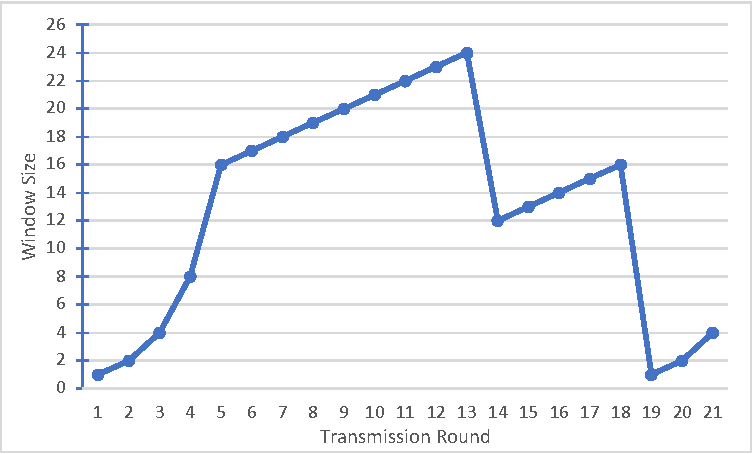
\includegraphics{figures/cc.pdf}
    \label{fig:cc}
\end{figure}

\begin{enumerate}
    \item At transmission round 13, was congestion detected by a timeout or duplicate ACKs?
    \item What is the threshold at transmission round 2?
    \item What is the threshold at transmission round 20?
    \item Suppose at transmission round 21, congestion is detected via duplicate ACKs. What will be the window size in transmission round 22?
    \item Suppose at transmission round 21, congestion is detected via duplicate ACKs. What will be the threshold in transmission round 22?
\end{enumerate}

\end{problem}

\subsection*{Answer 1:}
\begin{enumerate}
    \item At transmission round 13, congestion was detected by duplicate ACKs.
    \item The threshold at transmission round 2 is 16.
    \item The threshold at transmission round 20 is 8. 
    \item If the transmission round 21 detected congestion via duplicate ACKs, the window size in transmission round 22 would be 2.
    \item If the transmission round 21 detected congrestion via duplicate ACKs, the threshold in transmission round 22 would be 2.
\end{enumerate}
\begin{problem}{2: RED}
Recall from class that in the RED (Random Early Detect) scheme, packets can be dropped before the buffer is full. Suppose A is the running average of the number of packets in the buffer, and that w is the weight given to a new packet that arrives. When a new packet arrives, A is recalculated with the equation w*(current number of packets in buffer) + (1-w)*(A).
The probability of dropping a packet is given as:

\begin{equation}
p =
    \begin{cases}
        0 & \text{if } A < min\_thresh\\
        (A-5.0)/10.0 & \text{if } min\_thresh \leq A \leq max\_thresh \\
        1 & \text{if } max_thresh < A \\
     \end{cases}
\end{equation}

Suppose to start out that, there are 5 packets in the buffer, A = 4.9, w = 0.4, min\_thresh = 5 and max\_thresh = 7. For the first six packets that arrive, give the probability that each will get dropped. Among all arrivals, only packet 3 is actually dropped - the rest successfully reach the buffer, though your calculations may show that they have a non-zero probability of being dropped. Also assume that between packets 4 and 5, 1 packet is sent (i.e., removed from the buffer).  

\end{problem}
\subsection*{Answer 2: }
We can demonstrate each of our calculations and answers for the addition of each of the following packets. Before we add our first packet we can calculate A as follows,
\begin{align*}
    A = 0.4*(5) + (1-0.4)(4.9) = 4.94
\end{align*}
Which as $A < min\_thresh$, it follows that we add our first packet to the buffer.\\\\
Now, for our second packet, we can calculate $A$ as follows,
\begin{align*}
    A = 0.4(6) + (1-0.4)(4.94) = 5.364
\end{align*}
As $min\_thresh < A < max\_thresh$ we can see gives us a probability of $ (5.364- 5)/10 = 0.0364$ of being dropped. Thus, we can add our second packet to our buffer.\\\\
Now, for our third packet, we can calculate $A$ as follows,
\begin{align*}
    A = 0.4*(7) + (1-0.4)(5.364) = 6.0184
\end{align*}
As $min\_thresh < A < max\_thresh$, we can see gives us a probability of $(6.0184 - 5)/10 = 0.10184$ of being dropped.\\\\
Now, assuming that our packet was dropped, we can calculate $A$ for our 4th packet as follows,
\begin{align*}
    A = 0.4*(7) + (1-0.4)(6.0184) = 6.411
\end{align*}
As $min\_thresh < A < max\_thresh$, we can see gives us a probability of $(6.411 - 5)/10 = 0.1411$ of being dropped. Thus, we can add our packet to our buffer.\\\\
Now, assuming that one of our packets went through, we can now consider the situation for our 5th packet. We can calculate $A$ as follows,
\begin{align*}
    A = 0.4*(7) + (1-0.4)(6.411) = 6.65
\end{align*}
As $min\_thresh < A < max\_thresh$, we can see gives us a probability of $(6.65 - 5)/10 = 0.165$ of being dropped. Thus, we will add our packet to our buffer.\\\\
Now, assuming that our packets went through, we can now consider the situation for our 6th packet. We can calculate $A$ as follows,
\begin{align*}
    A = 0.4*(8) + (1-0.4)(6.65) = 7.19
\end{align*}
Which, as $A > max\_thresh$, we can see that we have a probability of 1 for dropping the packet and thus, packet 6 is not added to our buffer.

\begin{problem}{3: Token Buckets}
Suppose that we want to limit a particular flow to 2 Mbps in the long-term, with a maximum burst size of 6Mb, and that each token allows us to send 1Mb. The token bucket starts empty, and t=0 is the first time slot in which the token bucket starts receiving tokens. \\\\
Consider the following sequence of packet arrivals and determine in which time slot each packet is sent. Packets must be sent in the order they are received, and if there are insufficient tokens, we wait (i.e., we do not simply drop a packet if there aren't enough tokens). A packet can be sent in the same time slot in which it arrived if there are enough tokens, and tokens may be used in the same time slot in which they arrived. \\\\
At t=0, packet 1 (of size 2Mb) arrives at the buffer. \\
At t=1, packet 2 (of size 6Mb) arrives at the buffer. \\
At t=3, packet 3 (of size 2Mb) arrives at the buffer. \\
At t=5, packet 4 (of size 4Mb) arrives at the buffer. \\

\end{problem}
\subsection*{Answer 3:}
Assuming that $r = 2 \frac{Mb}{s}$, we can find that packet 1 is sent at time $t = 0$, packet 2 is sent at time $t = 3$, packet 3 is sent at time $t = 4$, and paclet 4 is sent at time $t = 5$.
\begin{problem}{4: Reading}
\href{https://par.nsf.gov/servlets/purl/10179370}{This} article summarizes recent work aimed at using machine intelligence for congestion control. Read the article and answer the following questions:

\begin{enumerate}
    \item Is machine learning a good fit for the congestion control problem? Why or why not?
    \item Of the challenges, which do you think is most concerning? Are there any other challenges you can think of that are not listed (it's fine if not)?
\end{enumerate}
\end{problem}
\subsection*{Answer 4:}
\begin{enumerate}
    \item It seems as though machine learning may be a good fit for the congestion control problem so long as different conditions are met and the conceerns are tampered. Due to the fact that it seems like a lot of behavior on a network is repeated over time and that common trends tend to develop as to traffic behavior, it would make sense that employing a ML algorithm would be useful. However, I agree with a number of the points that the article brings up especially with the unqiueness of many different networks and their behaviors which could make using a uniform ML model difficult to implement and implies that each network may need their own trained ML model which would be difficult and time consuming among the other difficulties brought up such as the issues with obtaining sufficient data.
    \item Of the challenges brough up, I think the most concerning is that these models have not really be implemented in real situations. I think that the fact that these methods have only been implemented in theory and not under "dynamic network conditions" can provide some questionability to the issues at hand. I also think that one other concern that we have discussed in class and that I did not see in the article was the fact that ML models are computationally intensive and can take time to run/bandwidth to run which is another question that I think could come up when trying to apply these models to congestion situations as these routing and congestion decisions have to made incredibly quickly.
\end{enumerate}

\begin{problem}{5}
How long did this assignment take you?
\end{problem}
\subsection*{Answer 5:}
This assignment took me $\approx 5$ hours.
\end{document}


